 \begin{frame}{Cumulative Scheduling}
\begin{itemize}
\item \texttt{disjunctive} is useful for \alert{unary} resources
\item It is actually a special case of \texttt{cumulative}
\begin{itemize}
\item I have $m$ copies of the same resource
\item No more than $m$ can be used at once!
\item Example: $m$ workers, $m$ bulldozers, $m$ tools, \ldots
\end{itemize}
\vspace*{2ex}

\item Assume task \texttt{t} takes \texttt{res[t]} resources
\end{itemize}

\tikzset{
    task/.style={rounded corners, minimum height=3.8ex,rectangle,anchor=south west},
    task1/.style={task,draw=black, top color=isseorange!5, bottom color=isseorange!30},    
    task2/.style={task,draw=black, top color=issegrey!5, bottom color=issegrey!30},
    task3/.style={task,draw=black, top color=BrickRed!5, bottom color=BrickRed!30},
}
 
%\vspace*{-6ex}
\begin{figure}
\begin{tikzpicture}[scale=1.0,x=1cm,y=1cm]
    % Draw axes
    \draw [<->,thick] (0,3.2) node (yaxis) [above] {\texttt{res[t]}}
        |- (5.5,0) node (xaxis) [right] {$t$};    

    \draw [<->,thick] (6,3.2) node (yaxis) [above] {\texttt{res[t]}}
        |- (11.5,0) node (xaxis) [right] {$t$};      
% first slide
 
    \node[task1,text width=1.8cm,text height=2cm] at (0,0) {  };        
    \node[task1,text width=2.3cm,text height=.5cm] at (0,2.25) { };         
    \node[task1,text width=2.5cm,text height=.2cm] at (2.05,0) {  }; 
    \node[task1,text width=1.cm,text height=.2cm] at (2.05,0.6) {  };         
   
    \node[task1,text width=1.8cm,text height=2cm] at (6,0) {  };        
    \node[task1,text width=2.3cm,text height=.5cm] at (8.05,1.2) { };         
    \node[task1,text width=2.5cm,text height=.2cm] at (8.05,0) {  }; 
    \node[task1,text width=1.cm,text height=.2cm] at (8.05,0.6) {  };    
  %  \node[task3] at (2,1.5) { cook spaghetti };  

\node at (1.9, 3.4) {\color{BrickRed} \Huge \Lightning };
	\node at (7.9, 3.4) {\color{ForestGreen} \Huge \checkmark };
	
	
 \draw [dashed,BrickRed,very thick] (-0.3,2.25) -- (11,2.25) ;
	   
\end{tikzpicture}
\end{figure}
\end{frame}

\begin{frame}[fragile]{Cumulative Global Constraint}



\begin{lstlisting}
predicate cumulative(array [int] of var int: s,
                       array [int] of var int: d,
                       array [int] of var int: r,
                       var int: b)
\end{lstlisting}

\begin{parchment}[MiniZinc Docs]
Requires that a set of tasks given by start times \texttt{s}, durations \texttt{d}, and resource requirements \texttt{r}, never require more than a global resource bound \texttt{b} at any one time.
\end{parchment}
\end{frame}


\begin{frame}[fragile]{Household Revisited}
How about buying a new computer? 
\begin{lstlisting}
predicate cumulative(array [int] of var int: s,
                       array [int] of var int: d,
                       array [int] of var int: r,
                       var int: b)
\end{lstlisting}

\begin{lstlisting}
set of TASK: conflicting = {codeAlfred, codeBen, workMother};
int: nComputers = 2;

constraint cumulative( [ s[t] | t in conflicting], 
                          [ d[t] | t in conflicting], 
                          [ 1   | t in conflicting], 
                          nComputers ); 
\end{lstlisting}

\end{frame}

\begin{frame}[fragile]{Solution (1 Computer)}

\begin{lstlisting}
int: readAlfred = 1; int: codeAlfred = 2;
int: readBen = 3; int: codeBen = 4; int: workMother = 5;
set of TASK: conflicting = {codeAlfred, codeBen, workMother};
array[TASK] of int: d = [5, 2, 3, 8, 12];
\end{lstlisting}
\small 
\begin{verbatim}
s = array1d(1..5 ,[0, 20, 0, 12, 0]);
e = array1d(1..5 ,[5, 22, 3, 20, 12]);
makeSpan = 22;
\end{verbatim}

\tikzset{
    task/.style={rounded corners, text centered, minimum height=3.8ex,rectangle,anchor=south west},
    task1/.style={task,draw=black, top color=isseorange!5, bottom color=isseorange!30},    
    task2/.style={task,draw=black, top color=ForestGreen!5, bottom color=ForestGreen!30},
    task3/.style={task,draw=black, top color=BrickRed!5, bottom color=BrickRed!30},
}
 \hspace*{-2ex}
 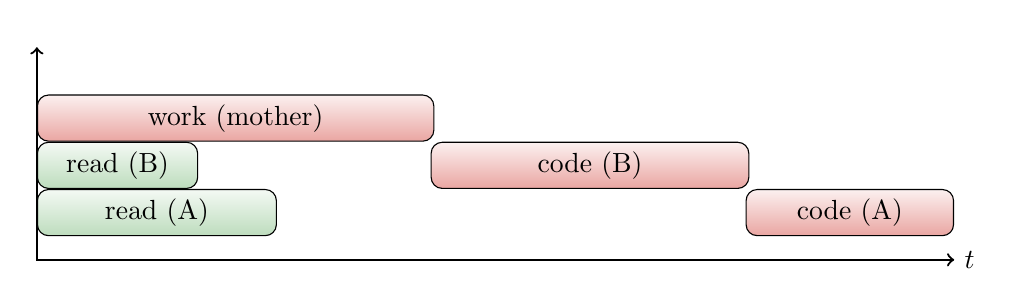
\begin{tikzpicture}[x=1cm,y=1cm]
    % Draw axes
    \draw [<->,thick] (0,2.7) node (yaxis) [above] {}
        |- (11.65,0) node (xaxis) [right] {$t$};    

  %  \node[task1] at (1,0.5) { cut onions };        
    \node[task2,text width=2.8cm] at (0,0.3) {read (A)};         
    \node[task2,text width=1.8cm] at (0,0.9) {read (B)};         

    \node[task3,text width=4.8cm] at (0,1.5) {work (mother)};         
	\node[task3,text width=2.4cm] at (9,0.3) {code (A)};         
    \node[task3,text width=3.8cm] at (5,0.9) {code (B)};        
   
  %  \node[task3] at (2,1.5) { cook spaghetti };  

\end{tikzpicture}
 
\end{frame}


\begin{frame}[fragile]{Solution (2 Computers)}

\begin{lstlisting}
int: readAlfred = 1; int: codeAlfred = 2;
int: readBen = 3; int: codeBen = 4; int: workMother = 5;
set of TASK: conflicting = {codeAlfred, codeBen, workMother};
array[TASK] of int: d = [5, 2, 3, 8, 12];
\end{lstlisting}
\small 
\begin{verbatim}
s = array1d(1..5 ,[0, 11, 0, 3, 0]);
e = array1d(1..5 ,[5, 13, 3, 11, 12]);
makeSpan = 13;
\end{verbatim}

\tikzset{
    task/.style={rounded corners, text centered, minimum height=3.8ex,rectangle,anchor=south west},
    task1/.style={task,draw=black, top color=isseorange!5, bottom color=isseorange!30},    
    task2/.style={task,draw=black, top color=ForestGreen!5, bottom color=ForestGreen!30},
    task3/.style={task,draw=black, top color=BrickRed!5, bottom color=BrickRed!30},
}
 \hspace*{-2ex}
 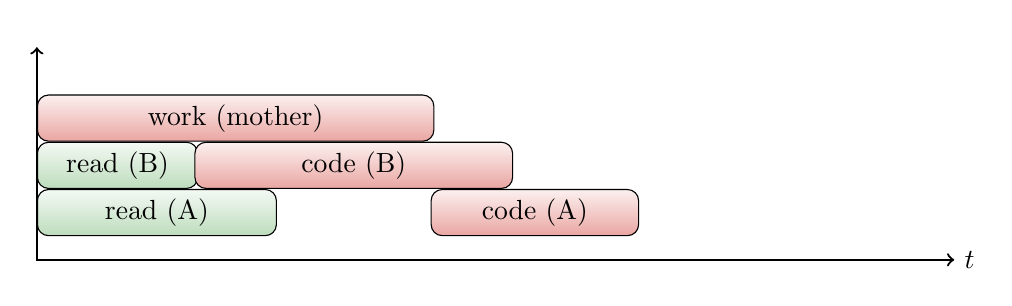
\begin{tikzpicture}[x=1cm,y=1cm]
    % Draw axes
    \draw [<->,thick] (0,2.7) node (yaxis) [above] {}
        |- (11.65,0) node (xaxis) [right] {$t$};    

  %  \node[task1] at (1,0.5) { cut onions };        
    \node[task2,text width=2.8cm] at (0,0.3) {read (A)};         
    \node[task2,text width=1.8cm] at (0,0.9) {read (B)};         

    \node[task3,text width=4.8cm] at (0,1.5) {work (mother)};         
	\node[task3,text width=2.4cm] at (5,0.3) {code (A)};         
    \node[task3,text width=3.8cm] at (2,0.9) {code (B)};        
   
  %  \node[task3] at (2,1.5) { cook spaghetti };  

\end{tikzpicture}
 
\end{frame}


